% Created 2010-06-02 Wed 13:04
\documentclass[11pt,a4paper]{report}
\usepackage[utf8]{inputenc}
\usepackage[spanish]{babel}
\usepackage{times}
\usepackage{amsmath}
\usepackage{amstext}
\usepackage{lscape}
\usepackage{color}
\setlength{\parindent}{7mm} %sangria la primera linea
\usepackage[pdftex=true,colorlinks=true,plainpages=false]{hyperref} % Soporte hipertexto

%PROFUNDIDAD DE LA TABLA DE CONTENIDO O ÍNDICE GENERAL
\setcounter{tocdepth}{4}
\setcounter{secnumdepth}{3}

\usepackage{graphicx}
\sloppy % suaviza las reglas de ruptura de líneas de LaTeX

\title{Stickmotion}
\author{grupo}
\date{Córdoba, 3 de Junio de 2010}

\begin{document}

\maketitle

\setcounter{tocdepth}{3}
\tableofcontents
\vspace*{1cm}






\chapter{Análisis de requisitos}
\label{sec-1}


\section{Introducción}
\label{sec-1.1}


Para clasificar y ordenar los requisitos es importante establecer una división de los distintos aspectos de la aplicación en diferentes bloques funcionales, permitiendo una descripción ordenada de lo que se espera del programa desarrollado. \\

\begin{figure}[htb]
\centerline{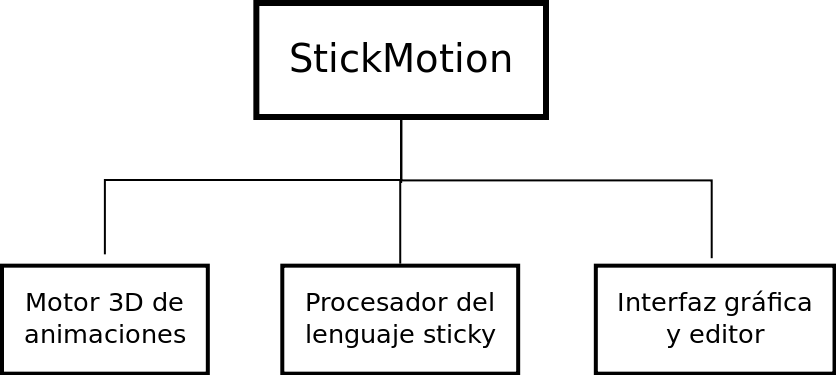
\includegraphics[width=\textwidth]{desc.funcional.png}}
\caption{\label{fig:dfuncional}Esquema de la descomposición en distintos bloques funcionales.}
\end{figure}


En la figura \ref{fig:dfuncional} se muestra un esquema de la descomposición funcional que se llevará a cabo. Los distintos bloques se describirán a continuación. \\

\subsection{Motor 3D de animaciones}
\label{sec-1.1.1}


Este bloque será el encargado de llevar a cabo la creación y gestión de la escena 3D, siendo el responsable del renderizado del Stickman que se deberá mostrar en la interfaz, así como realizar y almacenar las animaciones que se deberán realizar definidas por el lenguaje. \\

Deberá por tanto ofrecer una interfaz con funciones necesarias para la inclusión de animaciones en el Stickman, y obtener como salida una escena 3D que pueda ser mostrada en la interfaz gráfica. \\

\subsection{Procesador del lenguaje Sticky}
\label{sec-1.1.2}


Este bloque funcional será en cerebro de la interpretación del lenguaje Sticky diseñado, implementará las gramáticas empleando la librería ANTLR, y lo hará en base al lenguaje que se ha diseñado para tal efecto, al cuals e le ha denominado ``Sticky''.\\

Deberá por tanto recibir el código que sea introducido por el usuario y emplearlo procesando las acciones pertinentes para comunicarse con el motor 3D de animaciones en la realización de los movimientos que se especifiquen en el código Sticky. \\

\section{Requisitos funcionales}
\label{sec-1.2}


A continuación se enumerarán una serie de requisitos especificando las funciones que deberán realizar cada uno de los componentes en los que se ha dividido el diseño de la aplicación. \\

\subsection{Motor 3D de animaciones}
\label{sec-1.2.1}


\begin{itemize}
\item \textbf{RF1:} Deberá ofrecer la creación de una escena 3D que contenga la figura del Stickman.
\item \textbf{RF2:} La figura Stickman deberá poseer 4 extremidades y 1 cabeza que podrán rotarse en cualquier dirección del espacio tridimensional.
\item \textbf{RF3:} Cada una de las 4 extremidades del Stickman poseerá un punto de flexión sobre el cual podrá doblarse, en un ángulo dado (flexiones de antebrazos y antepiernas).
\item \textbf{RF4:} Para la animación deberá existir una linea temporal, por lo que deberá ofrecerse el manejo del tiempo como variable, pudiendo tanto accederse a su valor como modificarse.
\item \textbf{RF5:} Podrá especificarse la duración de cada movimiento de rotación o de flexión que se pretenda que realice el Stickman.
\end{itemize}
\subsection{Procesador del lenguaje Sticky}
\label{sec-1.2.2}


\begin{itemize}
\item \textbf{RF6:} Se seguirán las construcciones gramaticales, control de flujo y operaciones especificadas por la descripción del lenguaje Sticky.
\item \textbf{RF7:} Se ofrecerá una salida amigable en cuanto al reporte de errores, permitiendo en lo posible, la recuperación tras los mismos para continuar evaluando el resto del código.
\item \textbf{RF8:} Para facilitar la depuración, se ofrecerá un nivel regulable de detalle de la salida esperada, de forma que se muestren distintos mensajes de depuración o ``DEBUG'' si el usuario desea un mayor detalle sobre las operaciones que el procesador está realizando.
\end{itemize}
\subsection{Interfaz gráfica y editor}
\label{sec-1.2.3}


\begin{itemize}
\item \textbf{RF9:} Se podrá cargar archivos de código Sticky (extensión .stk) en la interfaz del editor.
\item \textbf{RF10:} Se podrá editar el código Sticky desde la propia interfaz del editor
\item \textbf{RF11:}
\item \textbf{RF12:} La interfaz ofrecerá un cuadro en el que se mostrará la escena 3D del Stickman en animación
\item \textbf{RF13:} La interfaz ofrecerá
\end{itemize}
\section{Requisitos no funcionales}
\label{sec-1.3}


Para poder llevar a cabo todos los objetivos correctamente nuestra aplicación deberá cumplir con la siguiente serie de requisitos no funcionales: \\


\begin{itemize}
\item \textbf{RNF1:} El programa deberá ser desarrollado en Java, siguiendo el programa de la asignatura, y ofreciendo además portabilidad en cuanto a plataforma de ejecución.
\item \textbf{RNF2:} El procesamiento del lenguaje deberá realizarse empleando la librería ANTLR para la creación de reconocedores de lenguaje.
\item \textbf{RNF3:} La aplicación deberá ofrecer un manejo intuitivo y sencillo.
\end{itemize}

\end{document}